\begin{figure}
     \centering
     \begin{subfigure}[b]{0.49\textwidth}
         \centering
         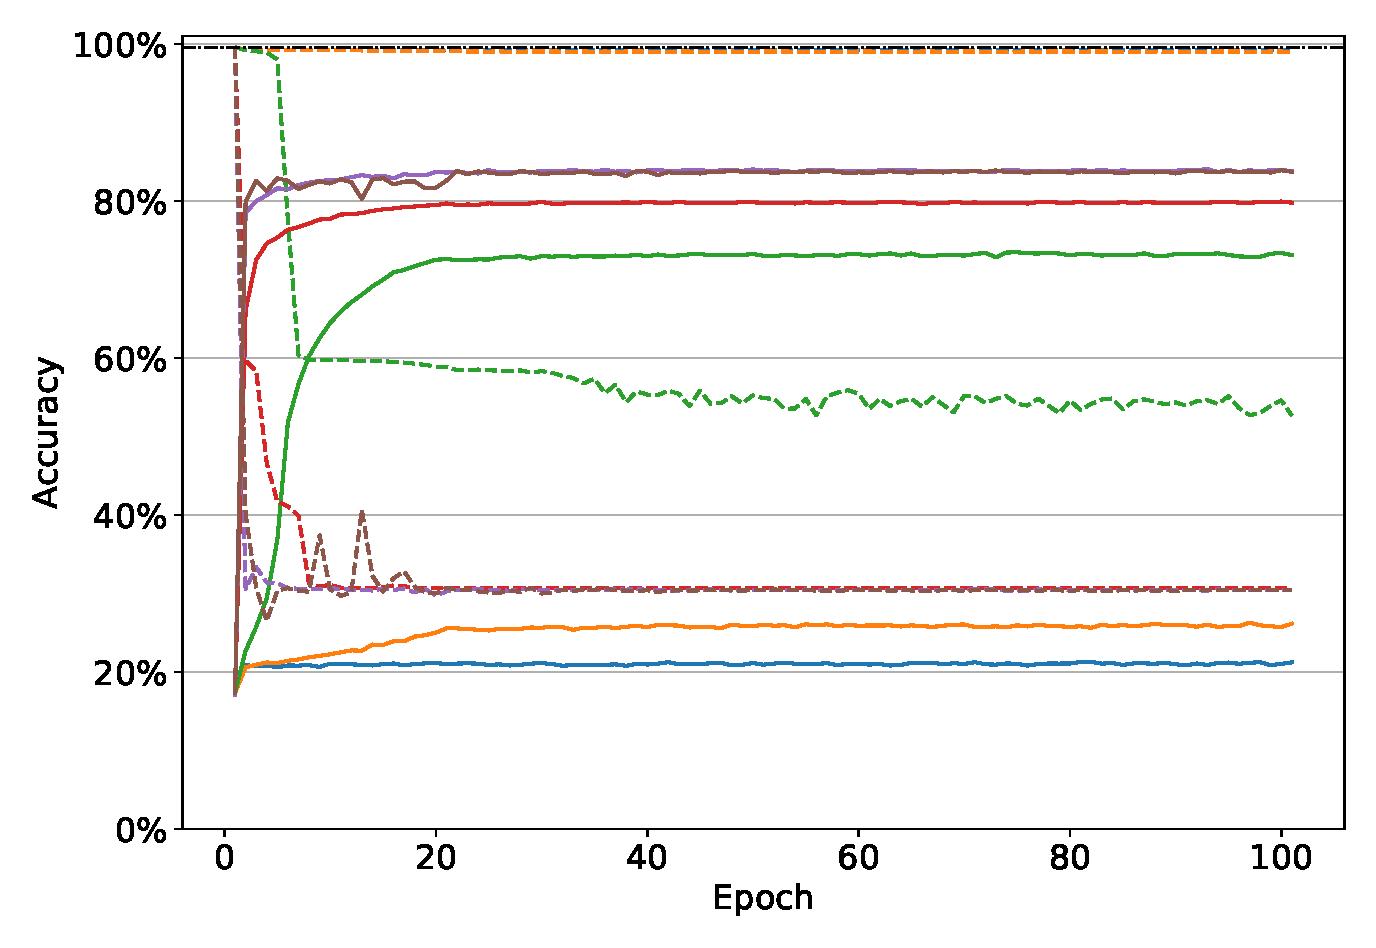
\includegraphics[width=\textwidth]{images/finetuning/finetuning_nonwm_model_thesis_simplenet_mnist_tunealllayers_False.eps}
         \caption{SimpleNet, only last layers}
         \label{fig:finetuning_simplenet_lastlayer}
     \end{subfigure}
     \hfill
     \begin{subfigure}[b]{0.49\textwidth}
         \centering
         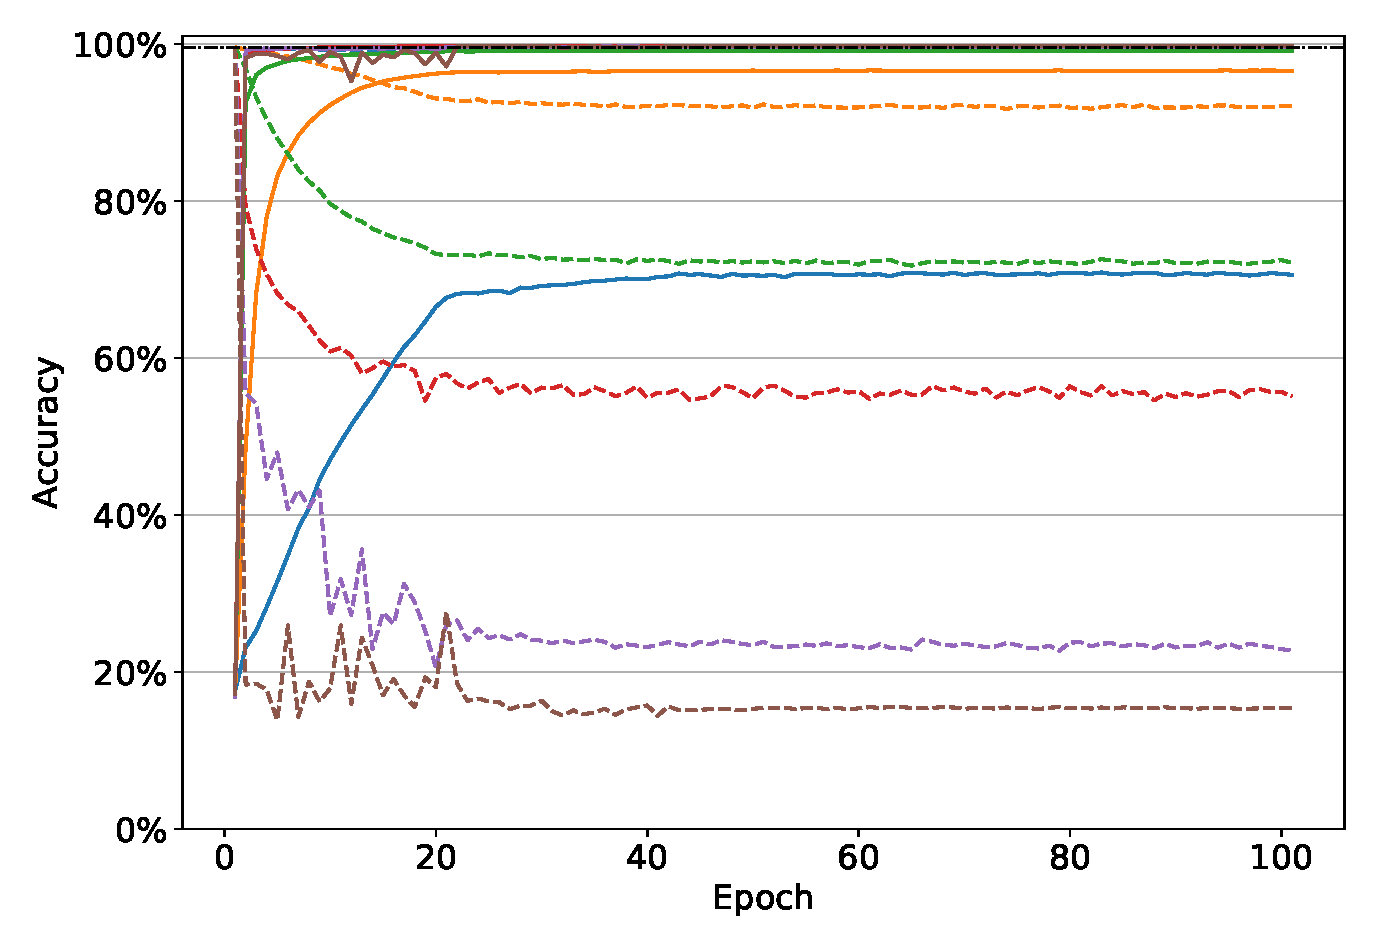
\includegraphics[width=\textwidth]{images/finetuning/finetuning_nonwm_model_thesis_simplenet_mnist_tunealllayers_True.eps}
         \caption{SimpleNet, all layers}
         \label{fig:finetuning_simplenet_alllayers}
     \end{subfigure}
     \hfill
     \begin{subfigure}[b]{\textwidth}
         \centering
         \includegraphics[height=1.1cm]{images/finetuning/legend_finetuning_allvslast_colors.eps}
         \quad
         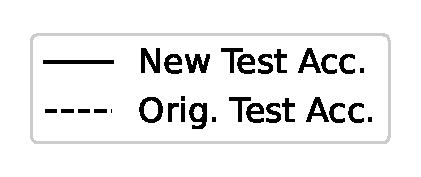
\includegraphics[height=1.1cm]{images/finetuning/legend_finetuning_allvslast_linetypes.eps}

     \end{subfigure}
     \caption{Fine-tuning on non-watermarked SimpleNet. The plot on the left side correspond to fine-tuning only the last layer and the one on the right hand side to fine-tuning all layers. The black dash-dotted line corresponds to the benchmark test accuracy of the non-watermarked model.}
     
     \label{fig:finetuning_all_vs_last_layers}
\end{figure}